\documentclass[main]{subfiles}

\begin{document}
\begin{lect}{2019-11-14}
    \begin{Reminder}
        \[(1) \qq\dot{x} = X(t, x) \qq \us{\text{обл}}{G} \subset \R^{n + 1} \]
        \[X \in C(G), \qq X \in \Lip_x^{loc}(G) \]
    \end{Reminder}

    %косяк
    \begin{Theorem}[3]
        (о поведении решения при приближении к концу макс.\\ промежутка задания)
        \[G \text{ - огр, }\q X \text{ - огр на } G\]
        \[x = \varphi(t) \text{ - реш } (1),\q t \in  (\alpha, \beta)
        \text{ макс промеж. задания } \varphi \]
        \[\Ra \exists \lim_{t \to \beta-} \varphi(t) = \xi,\q \text{ и }\q
        (\beta, \xi) \in \d G\]
    \end{Theorem}

    \begin{Proof}
        \[\delta > 0\]
        \[t_1, t_2 \in (\beta  - \delta, \beta)\]
        \[\varphi(t_1) = x_1 \Ra \varphi(t) \text{ уд З.К. } (t_1, x_1)\]
        \[\Ra \varphi(t) = x_1 + \int_{t_1}^t X(\tau, \varphi(\tau))d\tau \]
        \[\text{В частн., } \varphi(t_2) = x_1 + \int_{t_1}^{t_2}
        X(\tau, \varphi(\tau))d\tau\]
        \[\Ra \abs{\varphi(t_2) - \varphi(t_1)} = \abs{\int_{t_1}^{t_2}
        X(\tau, \varphi(\tau))d\tau} \leq \abs{\int_{t_1}^{t_2}
        \abs{X(\us{\leq M}{\tau, \varphi(\tau)})} d\tau }\]
        \[X \text{ - огр на } G \Ra \ \exists \  M : \ \abs{X(t, x)} \leq M, \qq
        \forall (t, x) \in G\]
        \[\Ra \abs{\varphi(t_2) - \varphi(t_1)} \leq M \cdot \abs{t_2 - t_1} \qq (2)\]
        \[\Ra \forall \mathcal{E} > 0 \q \exists \delta > 0 : \q \abs{t_2 - t_1}
        < \delta \ \Ra \  \abs{\varphi(t_2) - \varphi(t_1)} < \mathcal{E}\]
        \[\delta \leq \min(\beta - \alpha, \frac{\mathcal{E}}{M})\]
        \[\os{\text{кр. Коши}}{\Ra } \exists  \lim_{t \to \beta-} \varphi(t) = \xi \]
        \[\us{\forall t \in (\alpha, \beta)}{(t, \varphi(t))}
            \in G \ \Ra \ (\beta, \xi) \in \us{\text{замык}}{\overline{G}}\]
        \[\text{Если } (\beta, \xi) \in G \us{\text{Т1}}{\Ra} \varphi(t) \text{
        продолж. вправо за $\beta$ противореч.}\]
        \[\Ra (\beta, \xi) \in \overline{G} \setminus G = \d G\]
    \end{Proof}

    \begin{theorem} [3']
        Аналогичная $(3)$ для левого конца промежутка
    \end{theorem}


    \begin{Theorem}[о выходе макс. продолж. решения из компакта или Еругина]
        \[(1) \qq \dot{x} = X(t, x)\]
        \[x = \varphi(t) \text{ - реш. } (1) \qq t \in (\alpha, \beta)
        \text{ - макс. пр-к задания  } \varphi\]
        \[\us{\text{комп}}{D} \subset G\]
        \[\Ra \exists  \delta > 0 : \q\forall t \in (\beta - \delta, \beta) \qq
        (t, \varphi(t)) \ \cancel{\in }\ D\]
    \end{Theorem}

    \begin{Proof}[от противного]
        \[\us{\text{комп}}{D} \subset G \text{ - зафиксировали}\]
        \[\forall \delta > 0 \q \exists t \in (\beta - \delta, \beta): \q
        (t, \varphi(t)) \in D\]
        \[\{\delta_k\}_{k = 1}^\infty \qq \delta_k > 0  \qq \delta_1 > \delta_2 >
        ... > \delta_k > \delta_{k + 1} > ... \]
        \[\delta_k \us{k \to  + \infty}{\to } 0 \qq \delta_1 < \beta - \alpha\]
        \[\Ra \ \exists t_k : \q t_k \in (\beta - \delta_k, \beta) \text{ и }
        (t_k, \varphi(t_k)) \in \us{\text{комп}}{D}\]
        \[t_k \us{k \to  + \infty}{\to } \beta\]
        \[\exists  \text{ под/послед. } \{(t_k, \varphi(t_k))\}_{k = 1}^\infty,
        \text{ сх-ся  к } (\beta, \xi) \in D \subset G\]
        \[\Ra \exists  \ a > 0, \ b > 0: \]
        \[D_0 = \{(t, x) : \ \abs{t - \beta} \leq 2a, \ \abs{x - \xi} \leq 2b\}
        \subset G \qq\qq (3)\]
        \[X \in C(D_0) \ \Ra \exists M : \q \abs{X(t, x)} \leq M \q \forall (t, x)
        \in D_0\]
        \[h = \min\left(a, \frac{b}{M}\right)\]
        \[t_k \us{k \to +\infty}{\to }\beta \ \Ra \ \exists k_1 :\
        \forall k > k_1 \qq \beta - h < t_k < \beta \qq\qq(4)\]
        \[\varphi(t_k) \us{k \to  +\infty}{\to } \xi \Ra \exists k_2 : \
        \forall k > k_2 \qq \abs{\varphi(t_k) - \xi} < b \qq\qq (5)\]
        \[\text{фикс } k > \max(k_1, k_2) \ \Ra \ \text{ вып } (4), (5)\]
        \[D_k = \{(t, x): \ \abs{t - t_k} \leq a, \ \abs{x - \varphi(t_k)} \leq b\}\]
        \[\text{Докажем: } D_k \subset D_0\]
        \begin{figure}[H]
				    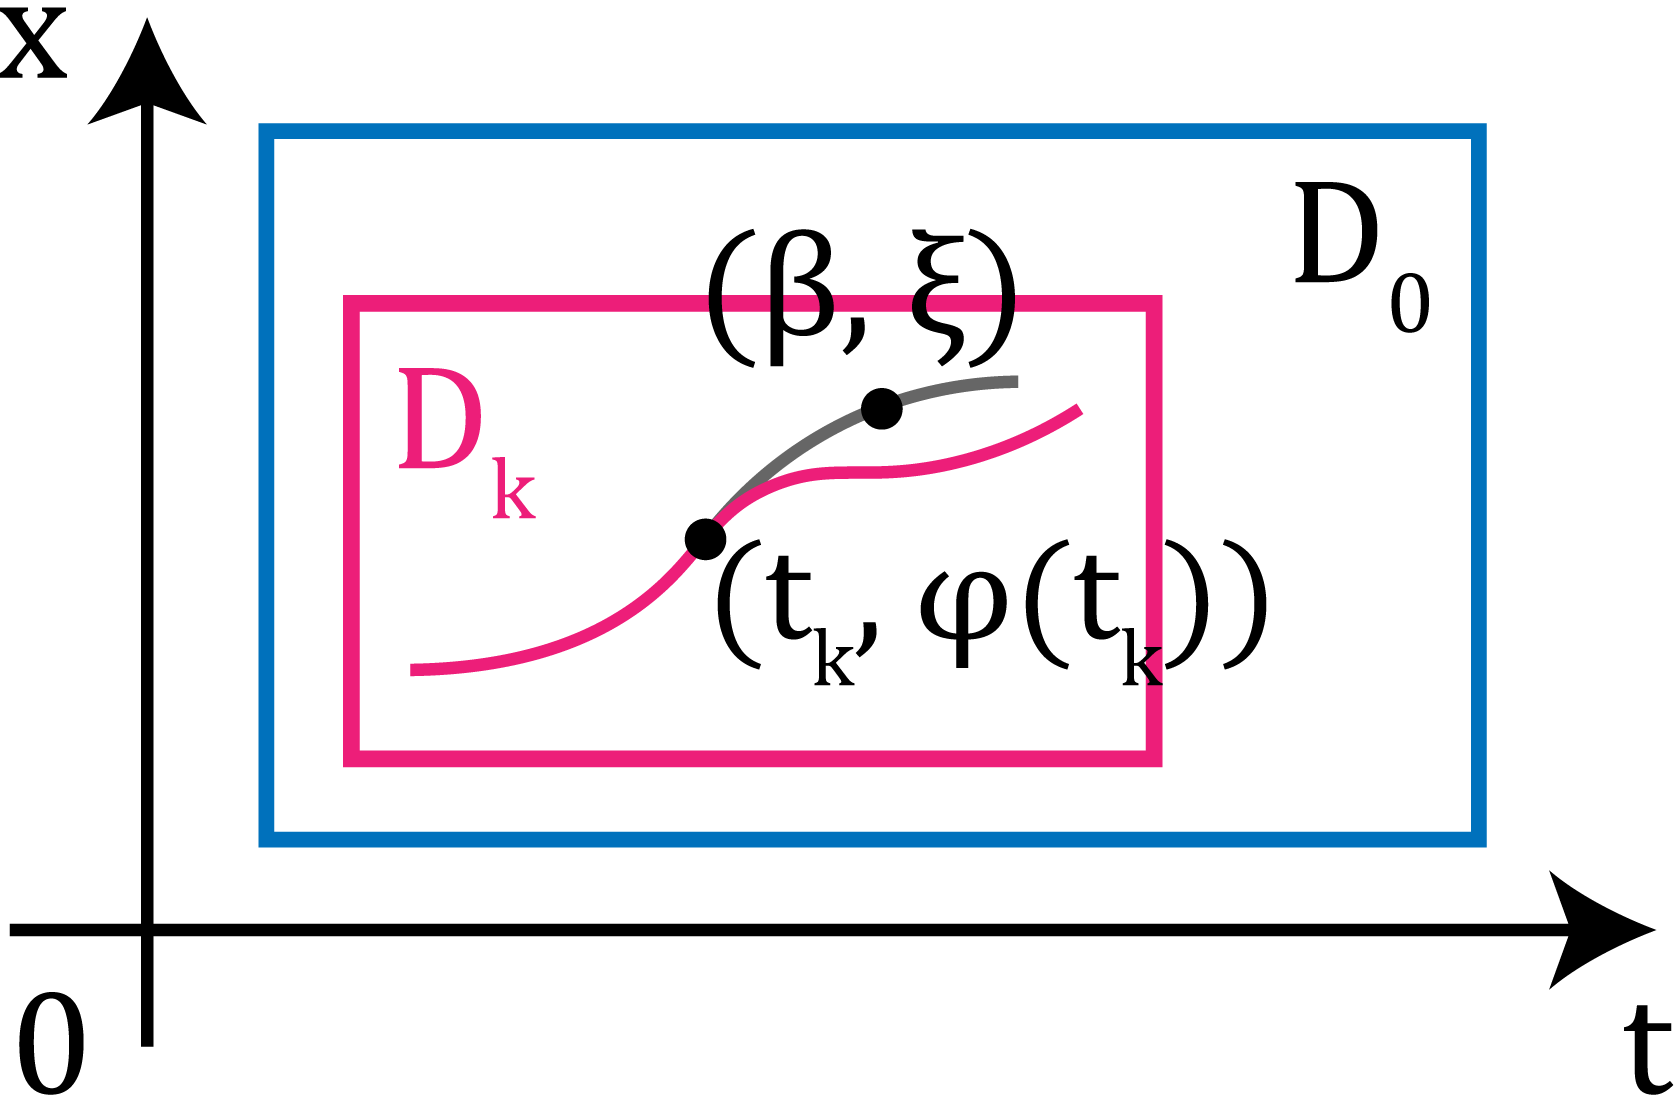
\includegraphics[width=4cm]{pics/10_1.png}
				    \centering
				\end{figure}
        \[\text{Взяли произвольную точку } \q (t, x) \in D_k\]
        \[\abs{t - \beta} \leq \abs{\us{\leq a}{t - t_k}} + \abs{\us{\leq h
        \leq a}{t_k - \beta}} \leq 2a\]
        \[\abs{x - \xi} \leq \abs{\us{\leq b}{x - \varphi(t_k)}}
        + \abs{\us{\leq b}{\varphi(t_k) - \xi}} \leq 2b\]
        \[\Ra (t, x) \in D_0\]
        \[\text{з. Коши } \q (t_k, \varphi(t_k))\]
        \[\exists \text{  реш } x = \psi(t), \text{ опред на } [t_k - h,\ t_k + h]\]
        \[\text{ и реш } x = \varphi(t) \q (t \in (\alpha, \beta)) \q
        \text{проходит через } (t_k, \varphi(t_k))\]
        %рисунок2 прямая с точками и отрезком
        \[\text{из (4)}: \ \beta < t_k + h\]
        \[x = \begin{cases}
            \varphi(t),& t \in (\alpha, \beta)\\
            \psi(t), & t \in [t_k - h,\ t_k + h]
        \end{cases} \text{ - продолжение } \varphi(t) \text{ вправо за } \beta\]
        противоречие\\
        (опред. корректно: $\varphi(t) \equiv \psi(t)$ на общ мн-ве)
    \end{Proof}

    \section{Системы сравнимые с линейными}

    \begin{Reminder}
        \[(1) \qq  \dot{x} = X(t, x) \qq X \in C(G), \q X \in \Lip_x^{loc}(G) \]
        \[G = \{(t, x) : \q t \in (a, b), \q x \in \R^n\} \qq \text{ м.б }
        a = -\infty \q b = -\infty\]
        \[\abs{x} < +\infty\]
    \end{Reminder}

    \begin{Definition}
        \[(1) \text{ - сравнима с линейной, если }\]
        \[\exists  \ M(t) \geq 0, \ N(t) \geq 0 \text{ - непрер. на } (a, b)\]
        \[(2) \q \abs{X(t, x)} \leq M(t) \cdot \abs{x} + N(t) \qq \forall t \in
        (a, b)\]
    \end{Definition}

    \begin{Theorem}
        \[(1) \text{ ср с лин.}\]
        \[x = \varphi(t) \text{ - реш. }(1) \ \Ra \ \varphi(t) \text{ опред на }
        (a, b)\]
    \end{Theorem}

    \begin{Proof}[от противного]
        \[\letus \ \exists \ \text{ решение (1) } x = \varphi(t), \text{ определена на }
        (\alpha, \beta) \text{ макс. пром. задания}\]
        \[(\alpha, \beta) \subset (a, b), \text{ но } (\alpha, \beta) \neq (a, b)\]
        \[\text{НУО } \beta < b:\]
        \[t_0 \in (\alpha, \beta) \q \varphi(t_0) = x_0\]
        \[\Ra \varphi(t) = x_0 + \int_{t_0}^t X(\tau, \varphi(\tau))d\tau \qq
        \forall t \in [t_0, \beta)\]
        \[\abs{\varphi(t)} \leq \abs{x_0} + \int_{t_0}^t \abs{X(\tau,
        \varphi(\tau))d\tau} \leq \abs{x_0} + \int_{t_0}^t N(\tau)d\tau +
        \int_{t_0}^t M(\tau)\abs{\varphi(\tau)}d\tau \]
        \[[t_0, \beta] \subset(a, b) \q (\beta < +\infty)\]
        \[M \text{ - непр на } [t_0, \beta] \ \Ra \ \exists  L > 0: \q
        \abs{M(t)} \leq L \qq \forall t_0 \in  [t_0, \beta]\]
        \[\int_{t_0}^t N(\tau)d\tau \leq \int_{t_0}^{\beta} N(\tau)d\tau  \]
        \[\Rightarrow \underset{\forall t \in \ [t_0, \beta)}{|\varphi(t)|} \leqslant
        \underbrace{|x_0|+\int_{t_0}^{\beta} N(\tau)d\tau}_{\text{c - const}} +
        L\int_{t_0}^{t} \varphi(\tau)d\tau\]
        \[\Rightarrow \text{ (Лемма Гронуолла) } |\varphi(t)| \leqslant ce^{L(t-t_0)} \leqslant
         ce^{L(\beta-t_0)} \ (3)\ \]
        \[D = \{(t, x) : t \in [t_0, \beta], \ |x| \ \leqslant \ ce^{L(\beta - t_0)} \} \text{из (3) следует, что }\]
        \[(t,\varphi(t)) \in \underbrace{D}_{\text{комп}} \forall t \in [t_0, \beta)
        \text{— противоречие с теорией о выходе макс. пр. реш-я.}\]
    \end{Proof}
\end{lect}
\end{document}
